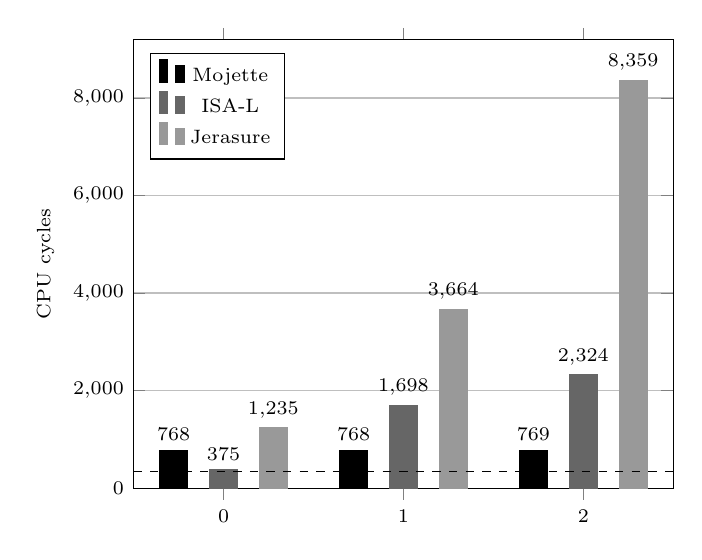
\begin{tikzpicture}
 \tikzstyle{every node}=[font=\scriptsize]
\begin{axis}[
    ybar=8pt,              % écarte les bars
    enlarge x limits=0.25,   % top ça ! écarte les côtés
    legend pos=north west,
    legend style={legend columns=1},
    ylabel={CPU cycles},
    %xlabel={Number of erasures},
    symbolic x coords={1,2,3},
    bar width=10pt,
    %x tick label style={ rotate=45 },
    %y tick label style={ rotate=90 },
    ymin=0,
    xtick={1,2,3},%
    xticklabels={0,1,2},
    error bars/.cd,
    yminorgrids=true,
    ymajorgrids=true,
    nodes near coords,
    cycle list = {black,black!60,black!40,black!10},
    %y filter/.code={\pgfmathparse{#1/336}\pgfmathresult}
    %scaled ticks=base 10:-3     %insane 
    %tick label style={/pgf/number format/fixed},
    %point meta=y *10^-7 % the displayed number
]

\addplot+[fill, text=black, error bars/.cd, y dir=both, y explicit]
 coordinates {
    (1,768)% +- (121,230)
    (2,768)%  +- (4,7)
    (3,769)% +- (18,27)
};
\addplot+[fill, text=black, error bars/.cd, y dir=both, y explicit]
coordinates {
    (1,375)% +- (20,32)
    (2,1698)%  +- (4,7)
    (3,2324)%  +- (2,4)
};
\addplot+[fill, text=black, error bars/.cd, y dir=both, y explicit]
coordinates {
    (1,1235)% +- (14,16)
    (2,3664)%  +- (4,7)
    (3,8359)%  +- (4,7)
};

\draw [black,dashed] ({rel axis cs:0,0}|-{axis cs:2,336}) -- ({rel axis cs:1,0}|-{axis cs:2,336}) node [pos=0.33, above] {};

\legend{Mojette, ISA-L, Jerasure}

\end{axis}
\end{tikzpicture}
